%!TeX root = RJwrapper.tex
%\begin{document} 
%\usepackage{multirow}

\title{\pkg{combinIT}: An R Package for Combining Interaction Tests for Unreplicated Two-Way Tables}
\author{by Mahmood Kharrati-Kopaei, Zahra Shenavari, Hossein Haghbin}
\maketitle

\abstract{
Several new tests have been proposed for testing interaction in unreplicated two-way analysis of variance models. Unfortunately, each test is powerful for detecting a pattern of interaction. Therefore, it is reasonable to combine multiple interaction tests to increase the power of detection for significant interactions. We introduce the package \CRANpkg{combinIT} that provides researchers the results of six existing recommended interaction tests, including: the value of test statistics, exact Monte Carlo p-values, approximated or adjusted p-values, the results of four combined tests and explanations of interaction types if the discussed tests are significant. The software \pkg{combinIT} is a more comprehensive R package in comparison with the two existing packages. In addition, the software is executed quickly to obtain the exact Monte Carlo p-values, even for large Monte Carlo runs, in contrast to existing packages.
}

\section{Introduction}\label{sec:introduction}
\noindent Suppose that there are two factors $A$ and $B$ with $a$ and $b$ levels, respectively. To investigate the effect of the factors on a response variable $y$, an unreplicated two-way analysis of variance (ANOVA) {model is sometimes used} to reduce the experiment cost. Formally, this model is 
\begin{equation} \label{eq:1}
	y_{ij}=\mu +\alpha_i+\beta _j+\gamma _{ij}+\epsilon_{ij},\ i=1,\dots ,a;\ \ j=1,\dots ,b,
\end{equation}
where $y_{ij}$ denotes the $i$-th and the $j$-th observation of the response variable, $\mu $ is the grand mean, $\alpha_i$ and $\beta_j$ denote the main effects of the factors, $\gamma_{ij}$s are interaction terms, and $\epsilon_{ij}$s are random errors which are independent and identically normal variables with mean zero and variance $\sigma^2$. As noted by \citet{Franck:2016}, the unreplicated two-way ANOVA models arise in the context of (a) completely randomized two-factor experiments, (b) randomized complete block experiments that block on a source of nuisance variability, and (c) observational studies with two factors. The main problem in an unreplicated two-way ANOVA model is that all observations are used to estimate the model parameters and no observations remain to estimate $\sigma^2$; see \citet{SKK:2018} and \citet{KKSA:2007}. Therefore, neither F-test nor t-test can be used to make inferences on the effects (including the interaction effect). The textbook approach is to assume that the interaction terms are zero (i.e. the model is additive). In this case, $\left(a-1\right)\left(b-1\right)$ degrees of freedom are left to estimate $\sigma^2$ and the usual F-tests can be used to make inferences about the main effects. However, if the interaction effects are present (i.e. the model is non-additive), the main effects may be masked by the interaction effect; see \citet{Montgomery:2017}. Therefore, it is important to implement some method to test if there exists a significant interaction in an unreplicated ANOVA model.

The existing approaches to test interaction in unreplicated two-way ANOVA models can be categorized into two main groups: functional-based-form (FBF) and non-functional-based-form (NFBF). In FBF approaches, a functional form is assumed for the interaction terms. This group includes interaction tests proposed by \citet{Tukey:1949}, \citet{Mandel:1961,  Mandel:1971}, \citet{JG:1972}, and \citet{CE:1972, CE:1974}; see \citet[pp 2--63]{MJ:1989} for a discussion of some of these interaction tests. \citet{SS:2013} also modified Tukey's test. It is known that these tests are powerful for detecting interaction only when the specified functional form for the interaction terms is appropriate; see \citet{Boik:1993}, \citet{AK:2006}, \citet{SS:2013}, and \citet{SKK:2018}. In NFBF approaches, a specific functional form is not assumed for the interaction terms. The NFBF group includes interaction tests proposed by \citet{MR:1977}, \citet{Tusell:1990}, \citet{Boik:1993}, \citet{Piepho:1994}, \citet{KKSA:2007}, \citet{Franck:2013}, \citet{Malik:2016} and \citet{KKM:2016}. \citet{KKSA:2007} formally showed that there does not exist the best interaction test in an unreplicated two-way ANOVA model in the sense that there is no test that can detect all patterns of interaction with high power. This means that {each test is powerful for detecting certain types of interaction}. Therefore, it is meaningful to combine multiple interaction tests to provide researchers with a testing approach that leverages many existing methods to detect different patterns of non-additivity. We note that the interaction tests are dependent and the main problem is how to combine multiple dependent tests into a single test procedure for testing additivity such that it controls the {Type I error} rate and has an acceptable power. \citet{SKK:2018} evaluated the performances of different combination methods and ultimately recommended combining the interaction tests by the Bonferroni method, a Beta (Sidak) approximation, the Jacobi polynomial expansion, and the Gaussian copula method. These methods are abbreviated as Bon, Sidak, JPE, and GC, respectively, throughout this paper.

Despite the application of unreplicated two-way ANOVA models in industry, biology, agriculture, and medicine, the newly proposed interaction tests have not been discussed in statistical packages; as similarly noted by \citet{Franck:2016}. Recently, \citet{Osborne:2016} released the package \CRANpkg{hiddenf} which is available from the Comprehensive R Archive Network (CRAN). As the name of the package \pkg{hiddenf} implies, this package mainly focuses on detecting a hidden non-additivity structure proposed by \citet{Franck:2013}. This package also reports the p-values of tests for non-additivity developed by \citet{Tukey:1949}, \citet{ Mandel:1961}, \citet{KKSA:2007}, and \citet{Malik:2016}. However, this package neither provides the result of NFBF interaction tests proposed in \citet{Boik:1993}, \citet{Piepho:1994}, and \citet{KKM:2016} nor the result of the combined interaction test. In addition, this package uses a Monte Carlo procedure to report the p-value of \citet{Malik:2016}; however, the applied procedure is rather time-consuming. Further, the package \pkg{hiddenf} provides only adjusted Bonferroni p-values of the tests proposed by \citet{KKSA:2007} and \citet{Franck:2013} instead of the exact Monte Carlo p-values. Although \citet{Franck:2016} mentioned that the Bonferroni adjustment is not overly conservative for $a \leq 7$, one might be interested in knowing the exact p-values. We note that \citet{SRS:2014} also developed the \CRANpkg{additivityTests} package that provides test statistics, critical values, and binary reject/fail-to-reject decisions for tests proposed by \citet{Tukey:1949}, \citet{Mandel:1961}, \citet{Boik:1993}, \citet{Tusell:1990}, \citet{JG:1972}, and \citet{SS:2013}. However, the \pkg{additivityTests} package does not provide the p-values of tests; see \citet{Franck:2016}.

In this paper, we introduce the R package \pkg{combinIT}, which is available from CRAN  \citep{SHKKN:2022}. This package reports both exact Monte Carlo and adjusted or approximate (if available) p-values of the six NFBF interaction tests developed by \citet{Boik:1993}, \citet{Piepho:1994}, \citet{KKSA:2007}, \citet{Franck:2013}, \citet{Malik:2016}, and \citet{KKM:2016}. We use abbreviations Boik, Piepho, KKSA, Franck, Malik, and KKM, respectively, for these NFBF tests. In addition, this package provides the results of four combined interaction tests that are based on the Bon, Sidak, JPE, and GC methods. Furthermore, if a significant interaction is detected by a combined test, the package \pkg{combinIT} gives some explanations of the interaction type or pattern. Note that FBF tests have not been considered in \pkg{combinIT} because \citet{Boik:1993b} showed that the Boik test is never less powerful and is sometimes much more powerful than the test proposed by \citet{JG:1972}, which can be regarded as an extension of FBF tests proposed by \citet{Tukey:1949} and \citet{Mandel:1961, Mandel:1971}. In addition, \citet{Boik:1993b} compared the Boik test with the NFBF test developed by \citet{Tusell:1990} and recommended the Boik test. Furthermore, the Piepho test is a modified version of the NFBF test proposed by \citet{MR:1977} hence this test has not been considered in \pkg{combinIT}, either. In summary, the \pkg{combinIT} package reports the results of all recommended existing interaction tests in unreplicated two-way ANOVA models and, in this view, can be regarded as a more comprehensive package than \pkg{hiddenf} for testing interaction. In terms of code execution speed, nearly 25\% of the code has been written in C++; see \url{https://github.com/haghbinh/combinIT}. We used the \CRANpkg{Rcpp} package \citep{RcppArticle1, RcppBook, RcppArticle2} for writing some parts of the codes in C++. Thus, Monte Carlo simulations for calculating the p-value of the Malik test are not as time-consuming as those in the \pkg{hiddenf} package. In addition, using the \pkg{Rcpp} package allows us to calculate the exact Monte Carlo p-values of the Franck and KKSA tests in a reasonable time, in contrast to the \pkg{hiddenf} package, which provides only adjusted Bonferroni p-values; see \citet{Franck:2016}.

The rest of the paper is organized as follows. In the next section, the six NFBF interaction tests and the four combination methods that are utilized in the \pkg{combinIT} package are briefly reviewed. Then, technical details of the \pkg{combinIT} package {are provided}. After that, use of the package \pkg{combinIT} is illustrated with an example. The execution speed of the code is also discussed in this section. Finally, the performances of the combined interaction tests in terms of controlling the {Type I error} rate are discussed via a simulation study by using the \pkg{hiddenf} and \pkg{combinIT} packages.

\section{Six NFBF interaction tests and four combination methods}
\noindent This section has two subsections. We first review the Boik, Piepho, KKSA, Franck, Malik, and KKM interaction tests. We also discuss what patterns of interactions these tests are {powerful for detecting}. We then review the Bon, Beta, JPE, and GC combination methods. These tests and combination methods are utilized in the \pkg{combinIT} package. Throughout this section, {the null hypothesis of interest} is $H_0:$ There is no interaction or, equivalently, $H_0: \gamma_{ij}=0$ for all $i$ and $j$ and $r_{ij}=y_{ij}-\bar{y}_{i.}-\bar{y}_{.j}+\bar{y}_{..}$ (in usual notation) denote the residuals of the model \ref{eq:1} under $H_0$.   

\subsection{Six NFBF interaction tests}
\noindent \strong{Boik.} Let $p=\text{min}\{a-1,b-1\}$, $q=\text{max}\{a-1,b-1\}$ and $\text{tr}\left(\mathbold{X}\right)$ denote the trace of matrix $\mathbold{X}$. \citet{Boik:1993} proposed a locally best invariant (LBI) test and $H_0$ is rejected when 
\[T_{\text{Boik}}=\text{tr}^{2}\left(\mathbold{R}^{\prime}\mathbold{R}\right)/\left(p\text{tr}\left(\left(\mathbold{R}^{\prime}\mathbold{R}\right)^2\right)\right) \]
is small, where $\mathbold{R}=[r_{ij}]$ denotes the residual matrix of the model \ref{eq:1}. \citet{Boik:1993} provided the exact distribution of the test statistic under the null hypothesis $H_0$ when $p=2$ and its asymptotic distribution when $q$ is large. Note that the p-value of the Boik test is always {1} when $p=1$. Note that { the \citet{Boik:1993} test is powerful for detecting} interaction when the matrix of interaction terms $[\gamma_{ij}]$ has small rank and one singular value dominates the remaining singular values; see \citet{Boik:1993b}. For example, the Boik test is powerful for detecting the multiplicative form of interaction. The package \pkg{combinIT} provides the value of test statistic $T_{\text{Boik}}$, an asymptotic p-value, and an exact p-value of the Boik test based on a Monte Carlo simulation procedure. 

\noindent \strong{Piepho.} \citet{Piepho:1994} discussed and modified an interaction test procedure proposed by \citet{MR:1977} by using the estimator of variance for each level of one factor; i.e.,
\[ \hat{\sigma}^2_{i}=\frac{a\left(a-1\right) W_{i}-\sum_{k=1}^a W_{k}}{\left(a-1\right)\left(a-2\right)\left(b-1\right)}, \]
where  $W_{i}=\sum_{j=1}^b r_{ij}^2$ . \citet{Piepho:1994} proposed three test statistics. The \pkg{combinIT} package utilizes the third one, which detects a significant interaction when
\[ T_{\text{Piepho}}=-\left(a-1\right)\left(a-2\right)\left(b-1\right)\log(U)/2 \]
is large, where $ U=2a \sum_{i<j} \hat{\sigma}^2_{i} \hat{\sigma}^2_{j}/\left(\left(a-1\right) \left(\sum_{i=1}^a \hat{\sigma}^2_{i}\right)^2\right)$. \citet{Piepho:1994} provided only an asymptotic chi-square distribution of $T_{\text{Piepho}}$ under $H_0$. By construction, the Piepho test is powerful for detecting interactions when the estimators of variances are heterogeneous across the levels of one factor. The package \pkg{combinIT} provides the value of test statistic $T_{\text{Piepho}}$, an asymptotic chi-square p-value, and an exact p-value of the Piepho test based on a Monte Carlo simulation procedure. 

\noindent \strong{KKSA.} Suppose that $a\geq b$ and $b \geq4$. Split the data table into two sub-tables, obtained by putting $a_1$ ($2\leq a_1 \leq a-2$) rows in the first sub-table and the remaining $a_2$ rows in the second sub-table ($a_1+a_2=a$). The number of all possible divisions of the data table is $\text{APD}=2^{\left(a-1\right)}-a-1$. For the $l$-th division, let RSS1 and RSS2 denote the residual sum of squares for the two sub-tables. Let $F_l^*=\text{max}\{F_l,1/F_l\}$ where $F_l=\left(a_2-1\right)RSS1/\left(\left(a_1-1\right)RSS2\right)$ and $P_l$ denote the corresponding p-value. \citet{KKSA:2007} proposed $\text{minP}=\min_{1\leq l \leq \text{APD}} P_l$  as a test statistic and the hypothesis of no interaction is rejected for a small value of $\text{minP}$. The KKSA test is powerful for detecting interaction when the magnitude of interaction effects is heteroscedastic across the sub-tables of observations. The package \pkg{combinIT} provides the value of the test statistic and an exact p-value of the KKSA test based on a Monte Carlo simulation procedure. In addition, it provides an approximate p-value based on the Bonferroni adjustment. Note that the KKSA test is not applicable when both $a$ and $b$ are less than {4}.
 
\noindent \strong{Franck.} \citet{Franck:2013} defined the hidden additivity structure as “the levels of one factor belong in two or more groups such that within each group the effects of the two factors are additive but the groups may interact with the ungrouped factor”. Based on this concept, \citet{Franck:2013} proposed a test statistic by dividing the table of data into two sub-tables and developing an interaction F-test. Then, they considered all possible configurations of data and used the maximum of the interaction F-tests as a test statistic; the all-configurations and maximum-interaction F-test (ACMIF). The hypothesis of no interaction is rejected when ACMIF is large. It is clear that the Franck test is powerful when there is a hidden additivity structure in the data set. The package \pkg{combinIT} provides the value of the test statistic (ACMIF), an exact p-value of the Franck test based on a Monte Carlo simulation procedure, and an approximate p-value based on the Bonferroni adjustment.

\noindent \strong{Malik.} \citet{Malik:2016} used the idea that some cells may be involved in a significant interaction pattern and those cells might produce large positive or negative residuals. Therefore, \citet{Malik:2016} proposed to partition
 the residuals into three clusters using a suitable clustering method like k-means clustering. The hypothesis of no interaction can be interpreted as the effect of the three clusters being equal. In more detail, \citet{Malik:2016} proposed the model
  $y_{ij}=\mu^{*}+\alpha_i^{*}+\beta_j^{*}+\xi_{k\left(ij\right)}+\epsilon_{ij}$ where $\xi_{k}$ is the cluster effect for the
   $k$-th cluster, $k=1, 2, 3$, and $k\left(ij\right)$ denotes the cluster $k$ to which the residual of the
$\left(i,j\right)$-th cell is assigned by the clustering procedure. \citet{Malik:2016} considered the hypothesis of no
interaction as $H_0: \xi_1=\xi_2=\xi_3$.
 Let $\text{SSE}\left(\text{cluster}\right)=\sum_{i=1}^a\sum_{j=1}^b\sum_{k=1}^3\left(y_{ij}-\hat{\mu}^{*}-\hat{\alpha}_i^{*}-\hat{\beta}_j^{*}-\hat{\xi}_{k\left(ij\right)}\right)^2$ 
 where the hat notation denotes the estimates of effects. \citet{Malik:2016} proposed the following test statistic to test
  $H_0$

\begin{equation*}
	T_{\text{Malik}}=\frac{\left(\sum_{i=1}^a\sum_{j=1}^b
		r_{ij}^2-\text{SEE}\left(\text{cluster}\right)\right)/2}{\text{SSE}\left(\text{cluster}\right)⁄\left(\left(a-1\right)\left(b-1\right)-2\right)}.
\end{equation*}
The hypothesis $H_0$ is rejected for large values of $T_{\text{Malik}}$. Note that the result of the Malik test may depend on the method of clustering. In the \pkg{combinIT} package, clustering is done by \ctv{kmeans} function in \CRANpkg{RcppArmadillo}. The \code{speed\textunderscore mode} parameter on the kmeans clustering was set as \code{static\textunderscore subset}. Note that the Malik test performs well when there are some cells that produce large negative or positive residuals due to significant interaction. The package \pkg{combinIT} provides the value of test statistic $T_{\text{Malik}}$ and an exact p-value of the Malik test based on a Monte Carlo simulation procedure.

\noindent \strong{KKM.} Let $\mu_{ij}=\mu +\alpha_i+\beta _j+\gamma _{ij}$ denote the $\left(i,j\right)$-th cell mean and let $\eta_{ij}=\mu_{ij}-\mu_{i^{\prime}j}-\mu_{ij^{\prime}}+\mu_{i^{\prime}j^{\prime}}, i\neq i^{\prime}; j \neq j^{\prime},$ denote pairwise interaction contrasts. \citet{KKM:2016} used the idea that if {a significant interaction is present}, its corresponding interaction contrast shall be significant. To describe this method, let $\mathbold{Z}$ be an $n\times 1$ vector with elements $y_{ij}-y_{i^{\prime}j}-y_{ij^{\prime}}+y_{i^{\prime}j^{\prime}}$ where $n=ab\left(a-1\right)\left(b-1\right)/4$ is the total number of estimated pairwise interaction contrasts. \citet{KKM:2016} proposed 
%\[ T_{\text{KKM}}=\max\{|Z_k|; k=1,…,n\}/\text{PSE} \]
as a test statistic, where $Z_k$ is the $k$-th element of $\mathbold{Z}$, $\text{PSE}=\text{median}\{|Z_k|; |Z_k|\leq 5S_0\}$ in which $S_0=\text{median}\{|Z_k|; k=1,…,n\}/c_0$ where $c_0$ is an unbiasing constant obtained by a Monte Carlo simulation. $H_0$ is rejected when $T_{\text{KKM}}$ is large. {This test procedure is powerful for detecting} significant interactions when they are caused by some cells; i.e. some values of $|Z_k|$ are large. The package \pkg{combinIT} provides the value of test statistic $T_{\text{KKM}}$ and the exact p-value of the KKM test based on a Monte Carlo simulation procedure.

\subsection{Four methods for combining interaction tests}
Since {there is no single best interaction test} in an unreplicated two-way ANOVA model, it is reasonable to combine multiple interaction tests to provide researchers with a testing approach that leverages many existing methods to detect different patterns of non-additivity. In this section, we review four combination methods that were proposed by \citet{SKK:2018}. Throughout the section, we assume that $K \geq 2$ tests, whose test statistics are dependent and whose distribution functions are continuous, have been performed for a null hypothesis $H_0$. Therefore, there are $K$ dependent p-values $P_1, \ldots, P_K$ corresponding to the interaction tests. We are going to combine these p-values into a single p-value using one of the following four test procedures for testing $H_0$.

\noindent \strong{Bon.} Following the Bonferroni inequality, $H_0$ can be rejected at level $\alpha$ when $Kp_{\text{min}}<\alpha$  where $p_{\text{min}}$ is the observed value of $P_{\text{min}}=\min_{1 \leq i \leq K} \{ P_i \}$. Note that the Bonferroni method leads to a \underline{conservative} method of combination; i.e. its {Type I error} rate is always less than $\alpha$; $\text{Pr}_{H_0}\{ KP_{\text{min}}<\alpha \} \leq \alpha$. 

\noindent \strong{Sidak.} The distribution function of  $P_\text{min}$ under $H_0$ would be a beta distribution with parameters $1$ and $K$ if $P_i, i=1, \ldots, K$, were independent; i.e. $\text{Pr}_{H_0} \{P_{\text{min}} \leq x \}=1-\left(1-x\right)^K$. When $P_i$s are dependent, it can be shown that there is an $x^{*}\in \left(0,1\right)$ such that $\text{Pr}_{H_0} \{P_{\text{min}} \leq x \} \leq 1-\left(1-x\right)^K$ for all $x < x^{*}$; see \citet{SAKK:2015}. Therefore, $H_0$ would be rejected at level $\alpha$ when $1-\left(1-p_\text{min} \right)^K<\alpha$. 

\noindent \strong{JPE.} The distribution of $P_{\text{min}}$ under $H_0$ can be approximated by the Jacobi polynomial expansion. In this expansion, the distribution of $P_{\min}$ is approximated by the weighted sum of several Beta distribution functions with parameters $p=1$ and $q=1/E_1-1$ where $E_1$ denotes the first moment of $P_{\min}$; see \citet{SKK:2018}. Up to the second term in the Jacobi polynomial expansion, the  distribution of $P_{\min}$ is approximated by a Beta distribution with parameters $1$ and $q$. In practice, the parameter $q$ can be estimated as $\hat{q}=\min \{ \max \{ 1,1/P_{\min}-1 \}, K-1 \}$; see \citet{SKK:2018}. By this approximation, the null hypothesis $H_0$ is rejected at level $\alpha$ when $1-\left(1-p_{\min}\right)^{\hat{q}}<\alpha$.

\noindent \strong{GC.} Let $Z_i=\Phi^{-1} \left(P_i\right)$, $i=1,\ldots ,K$, where $\Phi^{-1}\left(.\right)$ is the quantile function of the standard normal distribution. Although it is well known that $Z_i$s are marginally distributed as the standard normal distribution under the null hypothesis $H_0$, the joint distribution of the $Z_i$ is unknown in practice. One can use the Gaussian copula (GC) family to model the joint distribution of $Z_i$s. Therefore, one can assume that the random vector $\left(Z_1,\ldots,Z_K\right)$ has a $K$-variate normal distribution under the null hypothesis $H_0$ with zero mean vector and variance-covariance matrix $\mathbold\Sigma$. In this case, the null hypothesis $H_0$ is rejected at level $\alpha$ when
\[ \text{Pr}_{H_0} \{P_{\min} \leq p_{\min} \}=1-\text{Pr}_{H_0} \{ Z_1> \Phi^{-1}\left(p_{\min}\right), \ldots , Z_K> \Phi^{-1}\left(p_{\min}\right) \}< \alpha. \]
This probability is calculated by using \CRANpkg{mvtnorm} in the package \pkg{combinIT}. Note that $\mathbold{\Sigma}$ can be estimated by $\hat{\mathbold{\Sigma}}=\left(1-\hat{\rho}\right)\mathbold{I}_K+\hat{\rho}\mathbold{1}_K \mathbold{1}^{'}_K$ where $\mathbold{I}_K$ is a $K \times K$ identity matrix, $\mathbold{1}_K$ is a $K$-dimensional vector of ones, and $\hat{\rho}=\max \{-1/\left(K-1\right), 1-\sum_{i=1}^K \left(Z_i-\bar{Z}\right)^2/\left(K-1\right) \}$; see \citet{SKK:2018}.

\noindent \strong{Note 1.} If the null hypothesis $H_0$ is rejected, the combined tests can suggest a pattern of non-additivity by examining the interaction test for which $P_{\min}=\min_{1 \leq i \leq K} \{ P_i\}$ occurs.

\noindent \strong{Note 2.} The inequality $K p_{\min} \leq 1-\left(1-p_{\min}\right)^{K} \leq 1-\left(1-p_{\min}\right)^{\hat{q}}$ guarantees that the JPE method provides an interaction test that is never less powerful and is sometimes much more powerful than the Bon and Sidak counterparts. 

\section{Technical details about the \pkg{combinIT} package}
The \pkg{combinIT} package stands for "Combined Interaction Test". This package allows users to perform the six NFBF interaction tests individually and to perform a combined test of the six NFBF interaction tests. It also has a function to produce an interaction plot and four data sets. The available functions in the \pkg{combinIT} package are described in Table \ref{tab:1}. This package produces two S3-class objects: (i) ITtest, produced by functions that perform a single test and (ii) combtest, produced by the function that performs the combined test. These returned objects are lists with the following components: 
\begin{itemize}
	\item[(i)] \code{ITtest} class: For the return object of the functions \code{Malik\_test}, \code{Franck\_test}, \code{Boik\_test}, \code{KKSA\_test}, \code{KKM\_test}, and \code{Piepho\_test}.  An object of this class consists of a list of six components, including:
	\begin{itemize}
		\item[-] \code{pvalue\_exact}: The calculated exact Monte Carlo p-value. For \code{Boik\_test}, this is an exact Monte Carlo p-value when $p>2$ and it is an exact p-value for $p=2$. 
		\item[-] \code{pvalue\_appro}: For \code{Piepho\_test} this is an asymptotic p-value. This component is the Bonferroni-adjusted p-value for \code{Franck.test} and \code{KKSA\_test}. This component is not available for \code{Malik\_test} and \code{KKM\_test}. 
		\item[-] \code{nsim}: The number of Monte Carlo samples used to calculate the exact Monte Carlo p-values.
		\item[-] \code{statistic}: The value of the test statistic.
		\item[-] \code{data\_name}: The name of the input data set.
		\item[-] \code{test}: The name of the test.
	\end{itemize}
	\item[(ii)] \code{combtest} class: For the return object of the function \code{CI\_test}. An object of this class consists of a list of 19 components, including:
	\begin{itemize}
		\item[-]  \code{nsim}: The number of Monte Carlo samples used to calculate the exact Monte Carlo p-values.
		\item[-] \code{Piepho\_pvalue}: The p-value of Piepho's (1994) test.
		\item[-] \code{Piepho\_Stat}: The value of Piepho's (1994) test statistic.
		\item[-] \code{Boik\_pvalue}: The p-value of Boik test.
		\item[-] \code{Boik\_Stat}: The value of Boik's (1993) test statistic.
		\item[-] \code{Malik\_pvalue}: The p-value of Malik, et al.'s (2016)  test.
		\item[-] \code{Malik\_Stat}: The value of Malik, et al.'s (2016)  test statistic.
		\item[-] \code{KKM\_pvalue}: The p-value of Kharrati-Kopaei and Miller's (2016) test.
		\item[-] \code{KKM\_Stat}: The value of Kharrati-Kopaei and Miller's (2016) test statistic.
		\item[-] \code{KKSA\_pvalue}: The p-value of Kharrati-Kopaei and Sadooghi-Alvandi's (2007) test.
		\item[-] \code{KKSA\_Stat}: The value of Kharrati-Kopaei and Sadooghi-Alvandi's (2007) test statistic.
		\item[-] \code{Franck\_pvalue}: The p-value of Franck, et al.'s (2013) test.
		\item[-] \code{Franck\_Stat}: The value of Franck, et al.'s (2013) test statistic.
		\item[-] \code{Bonferroni}: The combined p-value by using the Bonferroni method.
		\item[-] \code{Sidak}: The combined p-value by using the Sidak method.
		\item[-] \code{Jacobi}: The combined p-value by using the Jacobi method.
		\item[-] \code{GC}: The combined p-value by using the Gaussian copula.
		\item[-] \code{data\_name}: The name of the input data set.
		\item[-] \code{test}: The name of the test.
	\end{itemize}
	
\end{itemize}

\begin{table}[h!]
	\centering
	%\small
	\fontsize{8.5}{12}\selectfont
	\begin{tabular}{m{1.6cm} >{\centering}m{2cm} m{5.8cm} m{3.5cm} }
		\toprule
		Function & Descriptions & \centering{Inputs} & \hspace{0.9cm}Main outputs  \\ 
		\midrule
		\code{Boik\_test} & Performs the Boik test  & The data matrix, the number of Monte Carlo samples for calculating the exact p-value. & The value of test statistic, an asymptotic p-value, the exact Monte Carlo p-value. \\  
		\midrule
		\code{Piepho\_test}     & Performs the Piepho test & The data matrix, the number of Monte Carlo samples for calculating an exact  p-value. & The value of test statistic, an asymptotic p-value, the exact Monte Carlo p-value. \\
		\midrule
		\code{KKSA\_test} & Performs the KKSA test & The data matrix, the number of Monte Carlo samples for calculating the exact p-value,  logical Elapsed\_time for printing the progress. & The value of test statistic, an adjusted p-value, the exact Monte Carlo p-value. \\
		\midrule  
		\code{Franck\_test}      & Performs the Franck test & The data matrix, the number of Monte Carlo samples for calculating the exact  p-value, logical Elapsed\_time for printing  the progress. & The value of test statistic, an adjusted p-value, the exact Monte Carlo p-value. \\
		\midrule  
		\code{Malik\_test}        & Performs the Malik test & The data matrix, the number of Monte Carlo samples for calculating the exact  p-value, logical Elapsed\_time for printing  the progress. & The value of test statistic and the exact Monte Carlo p-value. \\
		\midrule   
		\code{KKM\_test} & Performs the KKM test & The data matrix, the number of Monte Carlo samples for calculating the exact p-value and the unbiasing constant. & The value of test statistic and the exact Monte Carlo p-value. \\
		\midrule 
		\code{CI\_test} & Performs the six NFBF tests and their combined tests & The data matrix, the number of Monte Carlo samples for calculating the exact p-value and the unbiasing constant,  logical Elapsed\_time for printing  the progress. & The value of six test statistics, the exact Monte Carlo p-values of tests, and the result of four combined tests.\\  
		\midrule
		interaction\_plot & Plots the interaction plot & The matrix of data. & Interaction plot. \\
		\bottomrule   
	\end{tabular}
	\caption{A summary of the functions in the \pkg{combinIT} package .}
	\label{tab:1}
\end{table}


%\begin{table}[h!]
%	\centering
%	%\small
%	\fontsize{8.5}{12}\selectfont
%	\begin{tabular}{ >{\centering}m{1.7cm} >{\centering}m{2cm} m{3.5cm} m{3.5cm} %m{2cm}}
%		\toprule
%		Function & Descriptions & \centering{Inputs} & \hspace{0.9cm}Main outputs & %%C$++$ function(s) \\ 
%		\midrule
%		\code{Boik\_test} & Performs the Boik test  & The data matrix, the number of Monte Carlo samples for calculating the exact p-value. & The value of test statistic, an asymptotic p-value, the exact Monte Carlo p-value.& \code{Bfc}, \code{Bfsim} \\  
%		\midrule
%		\code{Piepho\_test}      & Performs the Piepho test & The data matrix, the number of Monte Carlo samples for calculating an exact  p-value. & The value of test statistic, an asymptotic p-value, the exact Monte Carlo p-value.& \code{piepoC}, \code{Pieposim} \\
%		\midrule
%		\code{KKSA\_test} & Performs the KKSA test & The data matrix, the number of Monte Carlo samples for calculating the exact p-value,  logical Elapsed\_time for printing the progress. & The value of test statistic, an adjusted p-value, the exact Monte Carlo p-value.& \code{kk\_f} \\
%		\midrule  
%		\code{Franck\_test}      & Performs the Franck test & The data matrix, the number of Monte Carlo samples for calculating the exact  p-value, logical Elapsed\_time for printing  the progress. & The value of test statistic, an adjusted p-value, the exact Monte Carlo p-value.&\code{hh\_f} \\
%		\midrule  
%		\code{Malik\_test}        & Performs the Malik test & The data matrix, the number of Monte Carlo samples for calculating the exact  p-value, logical Elapsed\_time for printing  the progress. & The value of test statistic and the exact Monte Carlo p-value.& \code{M\_f} \\
%		\midrule   
%		\code{KKM\_test} & Performs the KKM test & The data matrix, the number of Monte Carlo samples for calculating the exact p-value, the number of Monte Carlo samples for calculating the unbiasing constant. & The value of test statistic and the exact Monte Carlo p-value. & \code{PICfsim}, \code{C0}, \code{picf} \\
%		\midrule 
%		\code{CI\_test} & Performs the six interaction tests and the four combined tests & The data matrix, the number of Monte Carlo samples for calculating the exact p-value, the number of Monte Carlo samples for calculating the unbiasing constant,  logical Elapsed\_time for printing  the progress. & The value of six test statistics, the exact Monte Carlo p-values of tests, and the result of four combined tests. & \code{picf}, \code{hh\_f}, \code{kh\_f}, \code{bmp\_f}\\  
%		\midrule
%		interaction\_plot & Plots the interaction plot & The matrix of data. & Interaction plot.& \\
%		\bottomrule   
%	\end{tabular}
%	\caption{A summary of the functions in the \pkg{combinIT} package .}
%	\label{tab:1}
%\end{table}


 {The \code{print} method} is developed for a brief displaying of these objects. One of the key features of this package is to make it possible for users to obtain accurate results for various tests within a reasonable time. This feature was achieved by assigning the time-consuming parts of these tests to several C++ functions that are called from R using \pkg{Rcpp}. %These functions are shown in the last column of Table \ref{tab:1}.


\section{Using the package combinIT}
Here, we illustrate the usage of the \pkg{combinIT} package. We also compare the new package with \pkg{hiddenf} in terms of execution speed. For reference, the functions of \pkg{combinIT} have been shown in Table \ref{tab:1}. This table also presents some information about the inputs and outputs of functions. 

We consider the copy number variation (CNV) data set that contains CNV values for normal and tumor tissue samples among six dogs. In this data set, the value of CNV was measured as a signal intensity obtained from a comparative genomic hybridization (CGH) array, with higher signals corresponding to higher copy numbers; see \citet{Franck:2013} and \citet{Osborne:2016}. The following code loads the data and plots the interaction plot. It can be seen from Figure \ref{fig:1} that a hidden structure might exist (rows 4 and 5 are parallel and they interact with rows 1, 2, 3, and 6).

\begin{example}
	> library(combinIT)
	> data(CNV)
	> interaction_plot(CNV)
\end{example}

\begin{figure}[htbp]
	\centering
	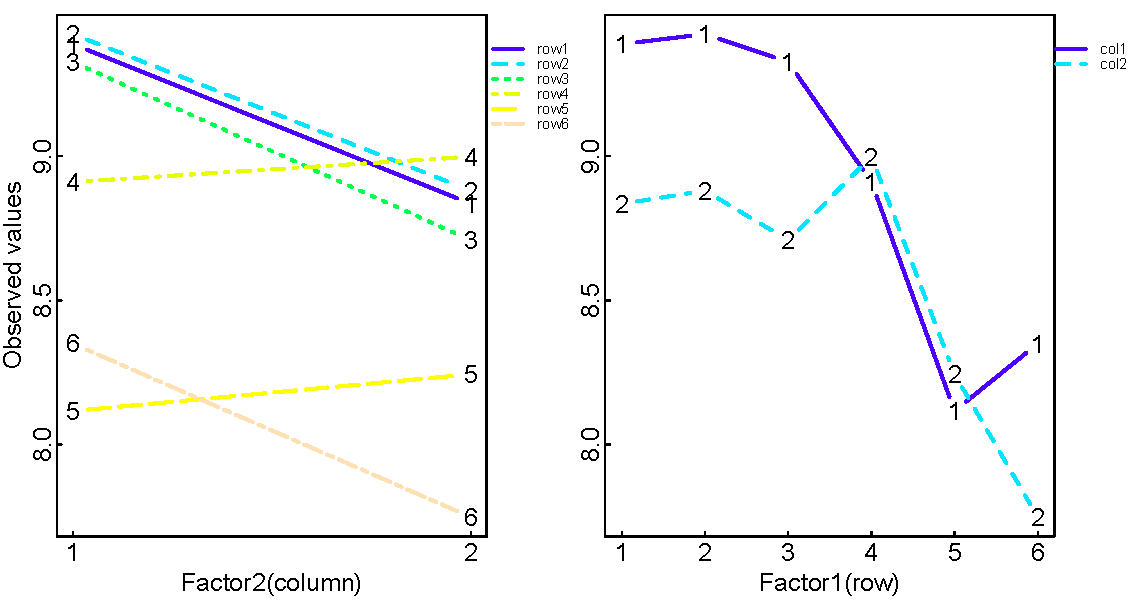
\includegraphics[width=14cm, height=6cm]{interactionplot1.pdf}
	\caption{The interaction plot of the CNV data.}
	\label{fig:1}
\end{figure}

Now, we use \code{CI\_test} to combine the result of the six interaction tests to see if there exists any significant interaction. We note that the exact Monte Carlo p-values are obtained based on 10000 Monte Carlo samples and hence the absolute error of Monte Carlo approximation is at most $0.0082$ with the 0.95 confidence coefficient (following the Central Limit Theorem). In addition, the p-value of the Boik test will be {1} since $p=1$. We also set $\alpha=0.05$ (as default to test at the 5\% level) and \code{report=TRUE} (to provide a report on the test), and \code{opvalue=0.6187} as the p-value of the Tukey's test (that is, we are going to combine the p-value of the Tukey's test in addition to the six interaction tests).

\begin{example}
	> CI_test(CNV, nsim = 10000, alpha = 0.05, report = TRUE, nc0 = 10000,
	opvalue = 0.6187, Elapsed_time = FALSE)
	Test:   Combined interaction Test 
	Data:   CNV 
	Piepho Test: Statistic =  1.73949 , Pvalue =  0.8743 
	Boik Test: Statistic =  1 , Pvalue =  1 
	Malik Test: Statistic =  526.66767 , Pvalue =  0.0289 
	KKM Test: Statistic =  1.18173 , Pvalue =  0.9994 
	KKSA Test: Statistic =  0.0112 , Pvalue =  0.2092 
	Franck Test: Statistic =  526.66767 , Pvalue =  7e-04 
	Bonferroni method: Pvalue = 0.0049 
	Sidak method: Pvalue = 0.00489 
	Jacobi method: Pvalue = 0.00419 
	Gaussian copula: Pvalue = 0.00491 
	------------------------------------------------ 
	A report on the combined interaction test:
	A  significant  hidden  structure  exists  at  the 5% level. The first
	group  includes  rows:  4, 5. The second group includes rows: 1, 2, 3,
	6.  The  estimated  critical  value of the Franck_test at the 5% level
	with 10000 Monte Carlo samples is 57.327.
 \end{example}

The \code{CI\_test} function has detected a significant interaction at the 5$\%$ level and the detected interaction type is the hidden structure as we expect. All combined tests report that there is a significant interaction. It is worth mentioning that a significant interaction would not be detected if only Boik or Piepho or KKM or KKSA test was used. However, the combined tests provide researchers with much more opportunity to detect a significant interaction. One can use the \code{Franck\_test} to analyze  the hidden structure in the CNV data set in more detail. The argument \code{plot} was set as \code{TRUE} to plot the interaction plot in the \code{Franck\_test} function. This interaction plot in Figure \ref{fig:2} shows that rows 4 and 5 are parallel (plotted in blue and solid line) and that they interact with rows 1, 2, 3, and 6 (plotted in red and broken line).  

\begin{figure}[htbp]
	\centering
	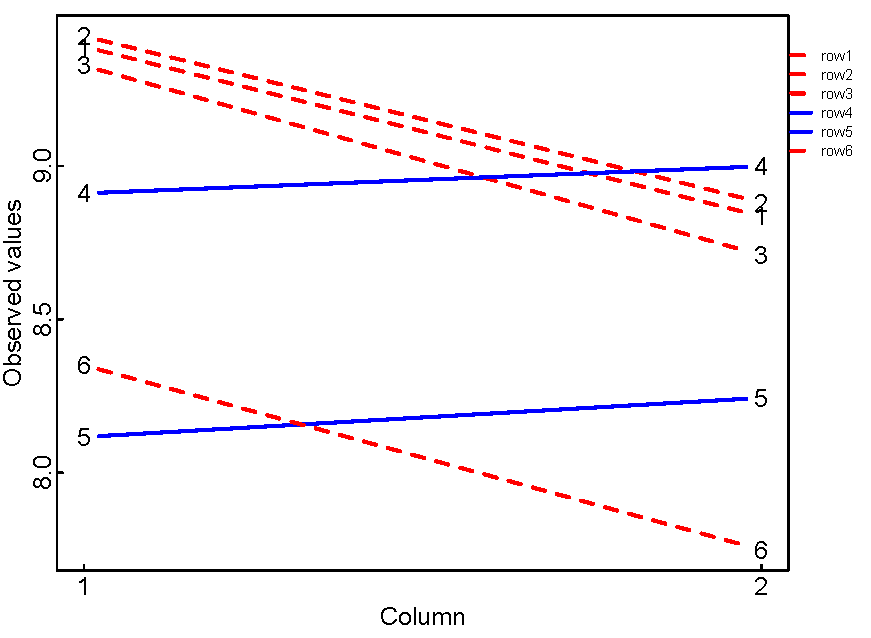
\includegraphics[scale=0.75]{interactionplot2.pdf}
	\caption{The interaction plot of the CNV data to see the hidden structure of interaction.}
	\label{fig:2}
\end{figure}

\begin{example} 
	> Franck_test(CNV, nsim = 10000, alpha = 0.05, report = TRUE, plot = TRUE,
	Elapsed_time = FALSE)
	Test:   Franck Test 
	Data:   CNV 
	Statistic =  526.668 
	Exact Monte Carlo P-value =  0 
	Approximate P-value =  0.001 
	Nsim =  10000 
	--------------------------------------- 
	A report on the test:
	A  significant  hidden  structure  exists  at  the 5% level. The first
	group  includes  rows:  4, 5. The second group includes rows: 1, 2, 3,
	6.  The  estimated  critical  value of the Franck_test at the 5% level
	with 10000 Monte Carlo samples is 56.7246. 
\end{example} 
 
Although the other five interaction tests can be used individually to test interaction, one should take care that a {Type I error} has not resulted from the multiple tests that have been performed. Code for each test is shown below.
   
\begin{example}
	> Boik_test(CNV, nsim = 10000, alpha = 0.05, report = TRUE)
	Test:   Boik Test 
	Data:   CNV 
	Statistic =  1 
	Exact Monte Carlo P-value =  1 
	Approximate P-value =  1 
	Nsim =  10000 
	--------------------------------------- 
	A report on the test:
	The  Boik_test  could not detect any significant interaction at the 5%
	level. The exact critical value of the Boik_test is 1. 
	> Piepho_test(CNV, nsim = 10000, alpha =0.05, report = TRUE)
	Test:   Piepho Test 
	Data:   CNV 
	Statistic =  1.739 
	Exact Monte Carlo P-value =  0.878 
	Approximate P-value =  0.884 
	Nsim =  10000 
	--------------------------------------- 
	 A report on the test:
	 The  Piepho_test  could  not detect any significant interaction at the
	 5%  level.  The  estimated critical value of the Piepho_test at the 5%
	 level with 10000 Monte Carlo samples is 12.5169. 
	> KKSA_test(CNV, nsim = 10000, alpha = 0.05, report = TRUE, plot = FALSE,
	Elapsed_time = FALSE)
	Test:   KKSA Test 
	Data:   CNV 
	Statistic =  0.011 
	Exact Monte Carlo P-value =  0.206 
	Approximate P-value =  0.28 
	Nsim =  10000 
	--------------------------------------- 
	 A report on the test:
	 The  KKSA_test  could not detect any significant interaction at the 5%
	 level.  The  estimated critical value of the KKSA_test at the 5% level
	 with 10000 Monte Carlo samples is 0.0023. 
	> Malik_test(CNV, nsim = 10000, alpha = 0.05, report = TRUE, Elapsed_time = FALSE)
	Test:   Malik Test 
	Data:   CNV 
	Statistic =  526.668 
	Exact Monte Carlo P-value =  0.026 
	Approximate P-value =  NULL 
	Nsim =  10000 
	--------------------------------------- 
	A report on the test:
	There   exists   a   significant   interaction  at  the  5%  level.The
	significant  interaction  might due to the some outliers in residuals;
	some cells produce large negative or positive residuals:
	The cell with row=5 and column=1 produces a large negative residual
	The cell with row=5 and column=2 produces a large positive residual
	The  estimated  critical  value of the Malik_test at the 5% level with
	10000 Monte Carlo samples is 362.0247.
	> KKM_test(CNV, nsim = 10000, alpha = 0.05, report = TRUE, nc0 = 10000)
	Test:   KKM Test 
	Data:   CNV 
	Statistic =  1.182 
	Exact Monte Carlo P-value =  0.999 
	Approximate P-value =  NULL 
	Nsim =  10000 
	--------------------------------------- 
	 A report on the test:
	 The  KKM_test  could  not detect any significant interaction at the 5%
	 level.  The  estimated  critical value of the KKM_test at the 5% level
	 with 10000 Monte Carlo samples is 4.2359. 
\end{example}

As we see, \code{{Boik\_test}}, \code{{Piepho\_test}}, \code{{KKSA\_test}}, and \code{{KKM\_test}} could not detect any significant interaction at the 5\% level. However, \code{{Malik\_test}} is significant and the significant interaction is due to the cells $\left(5,1\right)$ and $\left(5,2\right)$ that produce large negative and positive residuals, respectively. Note that the \code{{KKSA\_test}} has an argument \code{plot} that if \code{plot} is \code{TRUE} an interaction plot will be plotted. Color and line type are used to display which levels of row factor are assigned to which sub-tables based on the minimum p-values among all possible configurations. The values of the Monte Carlo p-value and the adjusted p-value of the Franck test {differ little} (the presented values were rounded up to three decimal digits and the actual value of the Monte Carlo p-value is around 0.00069){; on the other hand,} they differ for the KKSA test. This shows the importance of calculating the exact Monte Carlo p-values, while the package \pkg{hiddenf} provides only the adjusted p-values.

We now compare the {execution speed} of the \code{{Malik\_test}} function in the  \pkg{combinIT} package with the \code{MalikPavlue} function in the \pkg{hiddenf} package. To do this, we consider the CNV data again. We use the command \code{system.time} in R to record the elapsed time of execution in seconds for comparing the speed of execution. The elapsed time for 500 (the default of the \pkg{hiddenf} package), 1000, 5000, 10000 (the default of the \pkg{combinIT} package), 50000, and 100000 Monte Carlo samples are shown in Figure \ref{fig:3}. All computations were done on a laptop with \code{Windows 10} operating system, \code{Intel(R) Core(TM) i5-4200U CPU,1.60GHz 2.30 GHz} processor, and 8G of \code{RAM}. The following shows {the R code used} and the output for 500 Monte Carlo samples.
\begin{example}
	> library(hiddenf)
	> CNV.mtx<-HiddenF(CNV)
	> system.time(
	+ Malik_test(CNV,nsim=500,Elapsed_time = FALSE)
	+ )
	user  system elapsed 
	0.15    0.13    0.22 
	> system.time(
	+ MalikPvalue(CNV.mtx,N=500)
	+ )
	(Pvalue from Malik's test estimated with N=500 Monte Carlo datasets) 
	user  system elapsed 
	4.05    0.00    4.08 
\end{example}

\begin{figure}[tbp]
	\centering
	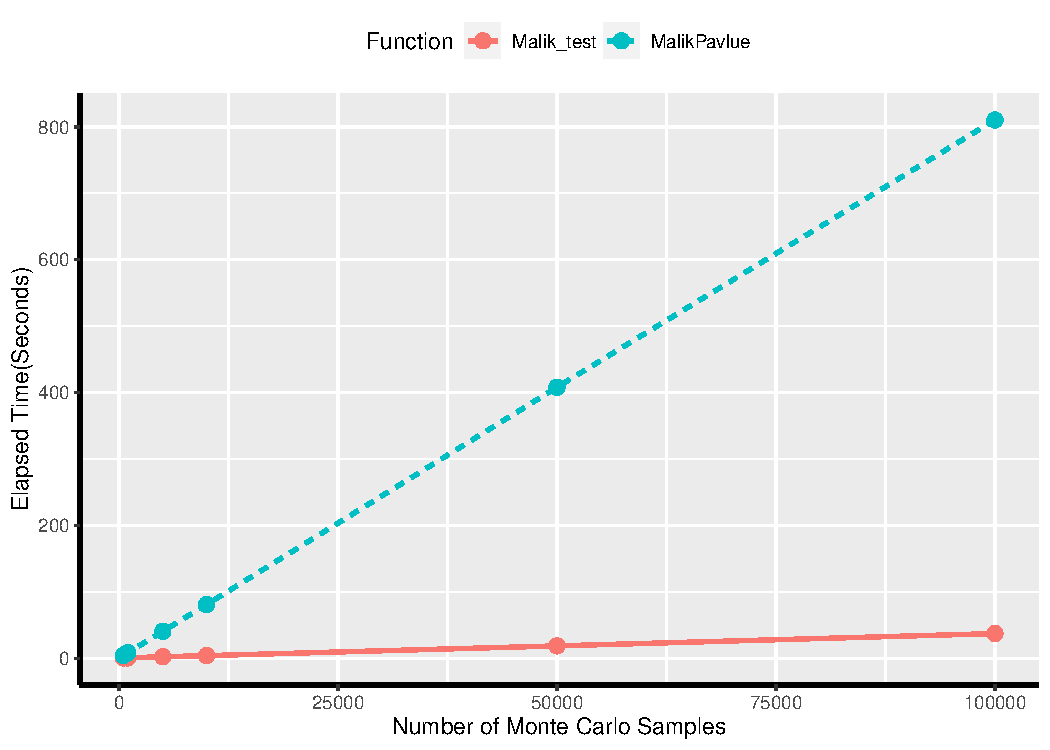
\includegraphics[scale=0.7]{elapsedtime.pdf}
	\caption{The elapsed time of executing \code{MalikPvalue} and \code{{Malik\_test}} functions for the CNV data.}
	\label{fig:3}
\end{figure}

It is seen that the {run time of the \code{{Malik\_test}} function is much shorter} than that of the \code{MalikPvalue} function. Actually, the run speed of the \code{{Malik\_test}} function is at least 18.5 times faster than the run speed of the \code{MalikPvalue} function.

\section{Simulation study}
In this section, we examine the performance of the Bon, Sidak, JPE, and GC methods in terms of controlling the {Type I error} rate using the \pkg{combinIT} and \pkg{hiddenf} packages. Note that \citet{SKK:2018} evaluated the performance of these {methods for combining the p-values of the Boik, Piepho, KKSA, Franck, KKM, and Malik tests}. Here, in addition to the six p-values, we consider the p-values {of Tukey's test} and Mandel's test \citep{Tukey:1949, Mandel:1961} as the two other tests that may apply. We used the following procedure to estimate the {Type I error} rate of the combination methods. For given $a$ and $b$, an $a\times b$ data table is generated from the standard normal distribution. We also took $\sigma^2=1$ without loss of generality (since the tests are scale invariant). For the computed interaction effects" changes to "For the generated data table, the tests are done and their p-values are recorded. For each method of combination, these p-values are combined and the result of the combined test's rejection of the null hypothesis of no interaction is recorded. This process is repeated $N1$ times and the fraction of times that the combined test rejects the null hypothesis is calculated as {an estimate of the Type} { I} error rate of the {combining} method. 

The results of simulation for $\alpha=0.10, 0.05, 0.01$, $N1=10,000$, and different values of $a$ and $b$ are shown in Table \ref{tab:2}. The exact Monte Carlo p-values of tests were calculated based on $N2=100,000$ Monte Carlo samples. In this table, the estimated absolute errors (EAE) {in} estimating the {Type I error} rate with confidence coefficient 0.95 are shown in parentheses. The value of EAE with confidence coefficient 0.95 is $1.96\sqrt{\hat{\alpha}\left(1-\hat{\alpha}\right)/N1}$ where $\hat{\alpha}$ denotes the estimated {Type I error} rate.

\begin{table}[h!]
	\centering
	%\small
	\fontsize{9}{12}\selectfont
	\begin{tabular}{>{\centering}m{1cm} >{\centering}m{1cm} >{\centering}m{1.7cm} >{\centering}m{1.7cm} >{\centering}m{1.7cm} m{1.7cm} }
		\cmidrule{3-6}
		&                   & \multicolumn{4}{c}{Methods} \\ 
		\midrule
		$\alpha$ & $a\times b$ & Bon & Sidak & JPE &  \hspace{0.5cm} GC \\  
		\midrule
		\multirow{4}[5]{*}{0.10} & $4\times3$ & 0.0681(0.0049) & 0.0716(0.0051) & 0.0822(0.0054) & 0.0770(0.0052)\\
		\cmidrule{2-6}
		& $5\times3$ & 0.0738(0.0051) & 0.0771(0.0052) & 0.0876(0.0055) & 0.0784(0.0054) \\
		\cmidrule{2-6}  
		&  $5\times5$& 0.0752(0.0052) & 0.0792(0.0053) & 0.0879(0.0055) & 0.0799(0.0053) \\
		\cmidrule{2-6}  
		& $6\times6$ &  0.0723(0.0051) & 0.0749(0.0052) & 0.0849(0.0055)  & 0.0764(0.0052) \\
		\midrule   
		\multirow{4}[5]{*}{0.05} & $4\times3$ & 0.0372(0.0037) & 0.0377(0.0037) & 0.0423(0.0039) & 0.0388(0.0038)\\
		\cmidrule{2-6}
		& $5\times3$  & 0.0384(0.0038) & 0.0394(0.0038) & 0.0441(0.0040) & 0.0396(0.0038) \\
		\cmidrule{2-6}  
		& $5\times5$ & 0.0399(0.0038) & 0.0411(0.0038) & 0.0463(0.0041) & 0.0406(0.0039)  \\
		\cmidrule{2-6}  
		& $6\times6$  &  0.0395(0.0038) & 0.397(0.0038) & 0.0448(0.0041) & 0.0402(0.0038)\\
		\midrule   
		\multirow{4}[5]{*}{0.01} & $4\times3$ & 0.0090(0.0019) & 0.0090(0.0019) & 0.0103(0.0020) & 0.0091(0.0019)\\
		\cmidrule{2-6}
		& $5\times3$ & 0.0078(0.0017) & 0.0078(0.0017) & 0.0088(0.0018) & 0.0079(0.0017) \\
		\cmidrule{2-6}  
		& $5\times5$ & 0.0090(0.0019) & 0.0092(0.0019) & 0.0101(0.0020) & 0.0092(0.0019) \\
		\cmidrule{2-6}  
		& $6\times6$ & 0.0087(0.0018) & 0.0087(0.0018) & 0.0096(0.0019) & 0.0086(0.0018) \\
		\bottomrule   
	\end{tabular}
	\caption{The estimated {Type I error} rates of the combined tests and their EAE (the values in parentheses).}
	\label{tab:2}
\end{table}

It is seen from Table \ref{tab:2} that the {combining} methods control the {Type I error} rate. This shows that these methods can be used for combining the p-values of the other tests successfully that {may be introduced} in the future. Among these four combination methods, the JPE method performs better than the others since the values of its estimated {Type I error} are fairly close to the nominal {Type I error}. We did not examine the performance of methods in terms of detecting a significant interaction power, because the considered methods do not have the same estimated Type I error rate (The JPE method would have the highest power, because its estimated Type I error rate is higher than the other methods; see also \strong{Note 2}).

\section{Summary}
We {reviewed six} recommended interaction tests in the context of unreplicated two-way ANOVA models and four combination methods for combining dependent interaction tests. Then, we introduced the \pkg{combinIT} package {and demonstrated that the} advantages of this package over the two existing packages are: (i) it reports test statistics, estimated critical value, approximate p-values, and exact Monte Carlo p-values {of six} recommended NFBF interaction tests, (ii) it provides the results of the four combined interaction tests in addition to some descriptions of detected significant interaction patterns, and (iii) its execution is fast enough to make it feasible to calculate the exact Monte Carlo p-values. Using the \pkg{combinIT} package, we evaluated the performance of the four combined tests in terms of controlling the {Type I error} rate. Simulation results show that the combined tests control the {Type I error} rate, and therefore can be used as an interaction test that leverages existing methods to detect different patterns of non-additivity.

We note that the \pkg{combinIT} package can handle data sets as large as $15\times15$, {although} performing the KKSA and Franck tests may be time-consuming when the size of the data set is larger. We will focus on solving this problem in {the next version of the package}. 

\section{Acknowledgment}
The first author would like to {acknowledge} the Research Council of Shiraz University.

\bibliography{Kharrati-Kopaei}

\address{Mahmood Kharrati-Kopaei\\
  Department of Statistics, College of Science, Shiraz University\\
  Shiraz\\
  Iran\\
  (ORCiD 0000-0001-5555-253X)\\
  \email{mkharati@shirazu.ac.ir}}

\address{Zahra Shenavari\\
	Department of Mathematics, Faculty of Sciences, Shiraz Branch, Islamic Azad University\\
	Shiraz\\
	Iran\\ 
	(ORCiD 0000-0001-8347-0590)\\
	\email{zshenavari@yahoo.com}}

\address{Hossein Haghbin\\
	Department of Statistics, Faculty of Intelligent Systems Engineering and Data Science, Persian Gulf University\\
	Boushehr\\
	Iran\\
	(ORCiD 0000-0001-8416-2354)\\
	\url{https://github.com/haghbinh}\\
	\email{haghbin@pgu.ac.ir}}
%\end{document} 
